\chapter{Investigating the Design of new CIPRNGs}
\label{CI dev}
\minitoc

In this chapter, some formerly proposed researches on CIPRNGs versions 1 and 2 are deepened. Then, in a second phase, the designs of our two brand new versions of pseudorandom number generators based on discrete chaotic iterations, and satisfying Devaney's chaos, are proposed and discussed. Detail operations of the proposed approach are described in this chapter, while their performance and  comparative studies will be presented in a next one. The works presented in this chapter have been formerly submitted in \cite{submit1, submit2, submit3}.



\section{Investigating the CIPRNG Version 1 Algorithm}

\subsection{On the periodicity of version 1}
\label{Conclusions and Future Work}
\label{Experiments and statistical tests}


As recalled in Section~\ref{Version 1 CI algorithms and examples}, the CIPRNG version 1, which is based on discrete chaotic iterations generated by two pseudorandom sequences ($m$ and $w$), has a long cycle length. Consider the default values for $\mathsf{N}$ and $m$, that is, $\mathsf{N}=4$ and $m \in \{$12,13$\}$. Let cycle period of $m$ and $w$ be respectively $n_m$ and $n_w$, the following part will analyze cycle period of version 1 sequence in greater depth.
Let us firstly recall the following definitions.
\begin{definition}%\cite{bahi102008}
A sequence $x = (x^{ 1} , ..., x^{n} )$ is said to be cyclic if a subset of successive terms is repeated from a given rank, until the end of $x$.
\end{definition}

\begin{definition}%\cite{bahi102008}
A sequence $x$ is said to be periodic with period $n$ if (for some nonzero constant $n$) we have
$$x^{k}=x^{k+n}$$
for all values of k. If there exists a least positive constant $n$ with this property, it is called the period. 
\label{period1}
\end{definition}

\begin{definition}
If a sequence $x$ is periodic with period $n$, then for all $k$ in the domain of $x$ and all integers $P$,
$$x^{k + nP} = x^{k}.$$
\label{period2}
\end{definition}

Having these definitions in mind, it is easy to prove that,
\begin{proposition}
Assume no value in the sequences $m$ and $w$ appears twice or more, and that $x^{k}=x^{k+n_x}$. If $m^{k}=m^{k+n_x/2}=m^{k+n_x}$ and $w^{\sum_{i=0}^{k-1}m_i}=w^{\sum_{i=0}^{k+n_x/2-1}m_i}=w^{\sum_{i=0}^{k+n_x-1}m_i}$(because $\bar{\bar{x}}=x$).
Then, $n_x=2n_wn_m$.
\end{proposition}
\begin{proof}
Let $a$ and $b$ be integers, and
$$w^{\sum_{i=0}^{k-1}m_i}=w^{\sum_{i=0}^{k+n_x/2-1}m_i}=w^{\sum_{i=0}^{k-1}m_i+\sum_{i=k}^{k+n_x/2-1}m_i},$$
$$m^{k}=m^{k+n_x/2}.$$
According to Definition \ref{period2}, we have
 \begin{equation}
\label{n_w}
\sum_{i=k}^{k+n_x/2-1}m_i=bn_w,
\end{equation}
\begin{equation}
\label{n_m}
n_x/2=an_m.
\end{equation}
From Eq. (\ref{n_m}), we can set Eq. (\ref{n_w}) that:
 \begin{equation}
\begin{array}{ll}
bn_w&=\sum_{i=k}^{k+n_x/2-1}m_i=\sum_{i=k}^{k+an_m-1}m_i=\sum_{i=0}^{an_m-1}m_i=\sum_{i=1}^{an_m}m_i,\\
&=a\sum_{i=1}^{n_m}m_i,\\
a&=bn_w/\sum_{i=1}^{n_m}m_i.\\
\end{array}
\end{equation}
For Definition \ref{period1}, $a$ and $b$ are least positive constants. Generally speaking, $\sum_{i=1}^{n_m}m_i>n_w$ ($m \in \{$12,13$\}$). If $\sum_{i=1}^{n_m}m_i$ and $n_w$ are coprime (also called relatively prime), we obtain:
$$a=n_w,$$
$$b=\sum_{i=1}^{n_m}m_i,$$
$$n_x=2n_wn_m,$$
which terminates the proof.
\end{proof}
Let us give an example for illustration purpose.
\begin{itemize}
\item $m \in \{$12,13$\}$ ($n_m=2$): 12,13,12,13 ...

\item $w \in \{$1,2$\}$ ($n_w=2$): 121212121212 1212121212121 212121212121 2121212121212 121212121212 1212121212121 212121212121 2121212121212...

\end{itemize}

In view of the above mentioned condition, the cycle will result in degeneration in normal circumstances as following. 

\begin{enumerate}
\item{\textbf{Rule 1}:} There is a greatest common divisor of $\sum_{i=1}^{n_m}m_i$ and $n_w$, which could be written as:
$$GCD=gcd(\sum_{i=1}^{n_m}m_i,n_w).$$
Then the cycle length is reduced to:
$$2n_wn_m/gcd(\sum_{k=1}^{n_m}m_i,n_w).$$
\item{\textbf{Rule 2}:} If the greatest common divisor of $\sum_{i=1}^{n_m}m_i$ and $n_w$ is not an even number, and $\sum_{i=1}^{n_m}m_i$ is an even number, the cycle length is then reduced to:
$$2n_wn_m/2=n_wn_m.$$
 \item{\textbf{Rule 3}:} All the  values in $w$ appear even times inside one cycle, such as
$$  w \in \{1,2\} (n=4):1221,$$ 
in which the values '1' and '2' appear twice inside the cycle. Then the cycle length is reduced to:
$$2n_wn_m/2=n_wn_m.$$
\end{enumerate}

To verify this method, let us consider $n_w=n_m=3$ and $n_w=n_m=4$ as study objects, as it is shown in Table~\ref{The cycle period with $n=3$}.
In that example, the greatest common divisor of $\sum_{k=0}^{n-1}m_k$ and $n$ is $1$, and due to $n=3$, the rule ``all values in $w$ appear even times'' is impossible. Then the only way to reduce the cycle length is by using the rule ``$\sum_{k=0}^{n-1} m_k (=38)$ is an even number''. Table~\ref{The cycle period with $n=4$} gives a closer look at how the rules work: it shows a special case in which Rule 1 and Rule 3 work together.


\begin{table}[!t]
\renewcommand{\arraystretch}{1.3}
\caption{The cycle period of the novel sequence with $n=3$}
\label{The cycle period with $n=3$}
\centering
  \begin{tabular}{|@{}c@{}|@{}c@{}|@{}c@{}|@{}c@{}|@{}c@{}|c|@{}c@{}|@{}c@{}|}
\toprule
$m$&$\sum_{k=0}^{n-1}m_k$&~GCD~&$w$&~even times~&one example for $x$&~Degeneration~&$n_x$\\\hline
\textbf{~(12,12,13)~~}& \multirow{3}{*}{37} &\multirow{3}{*}{1}&\multirow{6}{1.1cm}{\textbf{(1,1,2)}\\(1,1,3)\\(1,1,4)\\ \ldots \\ \ldots\\(4,4,1)\\(4,4,2)\\(4,4,3)}&\multirow{6}{*}{no}&\multirow{3}{2.5cm}{\textbf{(0,0,1,1,1,0,0,0,2,\\2,2,3,3,3,2,2,2,0)}}&&\multirow{3}{*}{~18~}\\
(12,13,12)& &&&&&&\\
(13,12,12)& &&&&&&\\\cline{1-3}\cline{6-8}
\textbf{(12,13,13)}& \multirow{3}{*}{38} &\multirow{3}{*}{1}&&&\multirow{3}{2.5cm}{\textbf{(0,1,0,0,2,3,3,2,0)}}&\multirow{3}{*}{\textbf{Rule 2}}&\multirow{3}{*}{9}\\
(13,12,13)& &&&&&&\\
(13,13,12)& &&&&&&\\
\bottomrule
  \end{tabular}
\\``one example for $x$'' illustrates the novel sequence depending on the sequences $m$ and $w$ in bolded text.
\end{table}

\begin{tiny}
\begin{sidewaystable}
\renewcommand{\arraystretch}{1.3}
\caption{The cycle period of the novel sequence with $n=4$}
\label{The cycle period with $n=4$}
\centering
  \begin{tabular}{||c||@{}c@{}|@{}c@{}|@{}c@{}|@{}c@{}|@{}c@{}||@{}c@{}|@{}c@{}|@{}c@{}|@{}c@{}|@{}c@{}||}
\toprule
Input sequences&$\sum_{k=0}^{n-1}m_k$&GCD&even times&Degeneration&$x_n$&$\sum_{k=0}^{n-1}m_k$&GCD&even times&Degeneration&$x_n$\\\hline\hline
\multirow{4}{*}{\backslashbox{\textbf{$w$}} {\textbf{$m$}}}&\multicolumn{5}{c||}{\textbf{(12,12,13,13)}}&\multicolumn{5}{c||}{others}\\\
&\multicolumn{5}{c||}{(12,13,13,12)}&\multicolumn{5}{c||}{\textbf{(12,12,12,13)}}\\
&\multicolumn{5}{c||}{(13,12,12,13)}&\multicolumn{5}{c||}{\ldots}\\
&\multicolumn{5}{c||}{(13,13,12,12)}&\multicolumn{5}{c||}{(13,13,13,12)}\\\hline\hline
\textbf{(1,1,2,2)} (1,1,3,3) (1,1,4,4) (1,2,2,1)&\multicolumn{5}{c||}{one example for $x$:\textbf{(0,0,1,0,0,0,2,0)}}&\multicolumn{5}{c||}{one example for $x$:\textbf{(0,0,0,1,1,1,1,0,0,0,0,2,2,2,2,0)}}\\\cline{2-11}
(1,1,2,2) (1,1,3,3) (1,1,4,4) (1,2,2,1)&\multirow{5}{*}{50}&\multirow{5}{*}{2}&\multirow{5}{*}{yes}&\multirow{5}{2cm}{\textbf{Rule 1}\\\textbf{Rule 3}}&\multirow{5}{*}{8}&\multirow{5}{1cm}{odd\\number}&\multirow{5}{*}{1}&\multirow{5}{*}{yes}&\multirow{5}{*}{\textbf{Rule 3}}&\multirow{5}{*}{16}\\
(1,1,2,2) (1,1,3,3) (1,1,4,4) (1,2,2,1)&&&&&&&&&&\\
(1,1,2,2) (1,1,3,3) (1,1,4,4) (1,2,2,1)&&&&&&&&&&\\
(1,1,2,2) (1,1,3,3) (1,1,4,4) (1,2,2,1)&&&&&&&&&&\\
(1,1,2,2) (1,1,3,3) (1,1,4,4) (1,2,2,1)&&&&&&&&&&\\\hline\hline
others&\multicolumn{5}{c||}{one example for $x$:\textbf{(3,0,2,0,3,0,2,3,0,3,1,3,0,3,1,0)}}&\multicolumn{5}{c||}{one example for $x$:\textbf{(3,0,3,1,2,1,2,0,3,0,3,1,2,1,2,3,}}\\
\multirow{3}{*}{\textbf{(1,1,1,2)}\ldots(4,4,4,3)}&\multicolumn{5}{c||}{}&\multicolumn{5}{c||}{\textbf{0,3,0,2,1,2,1,3,0,3,0,2,1,2,1,0)}}\\\cline{2-11}
&\multirow{2}{*}{50}&\multirow{2}{*}{2}&\multirow{2}{*}{no}&\multirow{2}{*}{\textbf{Rule 1}}&\multirow{2}{*}{16}&odd&\multirow{2}{*}{1}&\multirow{2}{*}{no}&&\multirow{2}{*}{32}\\
& & & & &&number&&&&\\
\bottomrule
  \end{tabular}
``one example for $x$'' illustrates the novel sequence depending on the sequences $m$ and $w$ in bolded text.
\end{sidewaystable}
\end{tiny}

If the final output is a 32-bit integer, then 8 4-bit outputs of the CIPRNG version 1 create a 32-bit integer, so
$n_{x_{32}}=LCM(n_{x_4},8)/8,$
where LCM is the least common multiple.
As a comparison, Table~\ref{The ideal cycle period} gives the ideal cycle period of various 32-bit generators.
\begin{table}
\renewcommand{\arraystretch}{1.3}
\caption{Ideal cycle period}
\label{The ideal cycle period}
\centering
% \begin{tiny}
\begin{tabular}{|c|c|c|}\toprule\hline
\multicolumn{2}{|c|}{\textbf{PRNG}}&\textbf{Ideal cycle period}\\\hline
\multicolumn{2}{|c|}{\textbf{XORshift}}&$2^{32}-1$ \\\hline
\multicolumn{2}{|c|}{\textbf{ISAAC}}& $2^{8295}$\\\hline
\multirow{3}*{\textbf{CIPRNGs version 1}}&\textbf{XORshift+XORshift}&$(2^{32}-1)^2$\\\cline{2-3}
&\textbf{XORshift+ISAAC}&$(2^{32}-1)~2^{8293}$\\\cline{2-3}
&\textbf{ISAAC+ISAAC}&$2^{16588}$\\\hline
\bottomrule
\end{tabular}
% \end{tiny}
\end{table}
\medskip

The schematic view of a typical orbit of a digital chaotic system is shown in Fig.\ref{A pseudo orbit of a digital chaotic system}. Generally speaking, each digital chaotic orbit includes two connected parts: $x^{0} , x^{1} , \dots, x^{l-1}$ and $ x^{l} , x^{l +1} , \dots , x^{l +n}$ , which are respectively called transient (branch) and cycle. Accordingly, $l$ and $n + 1$ are respectively called transient length and cycle period, and $l + n$ is called orbit length. 

\begin{figure}
\centering
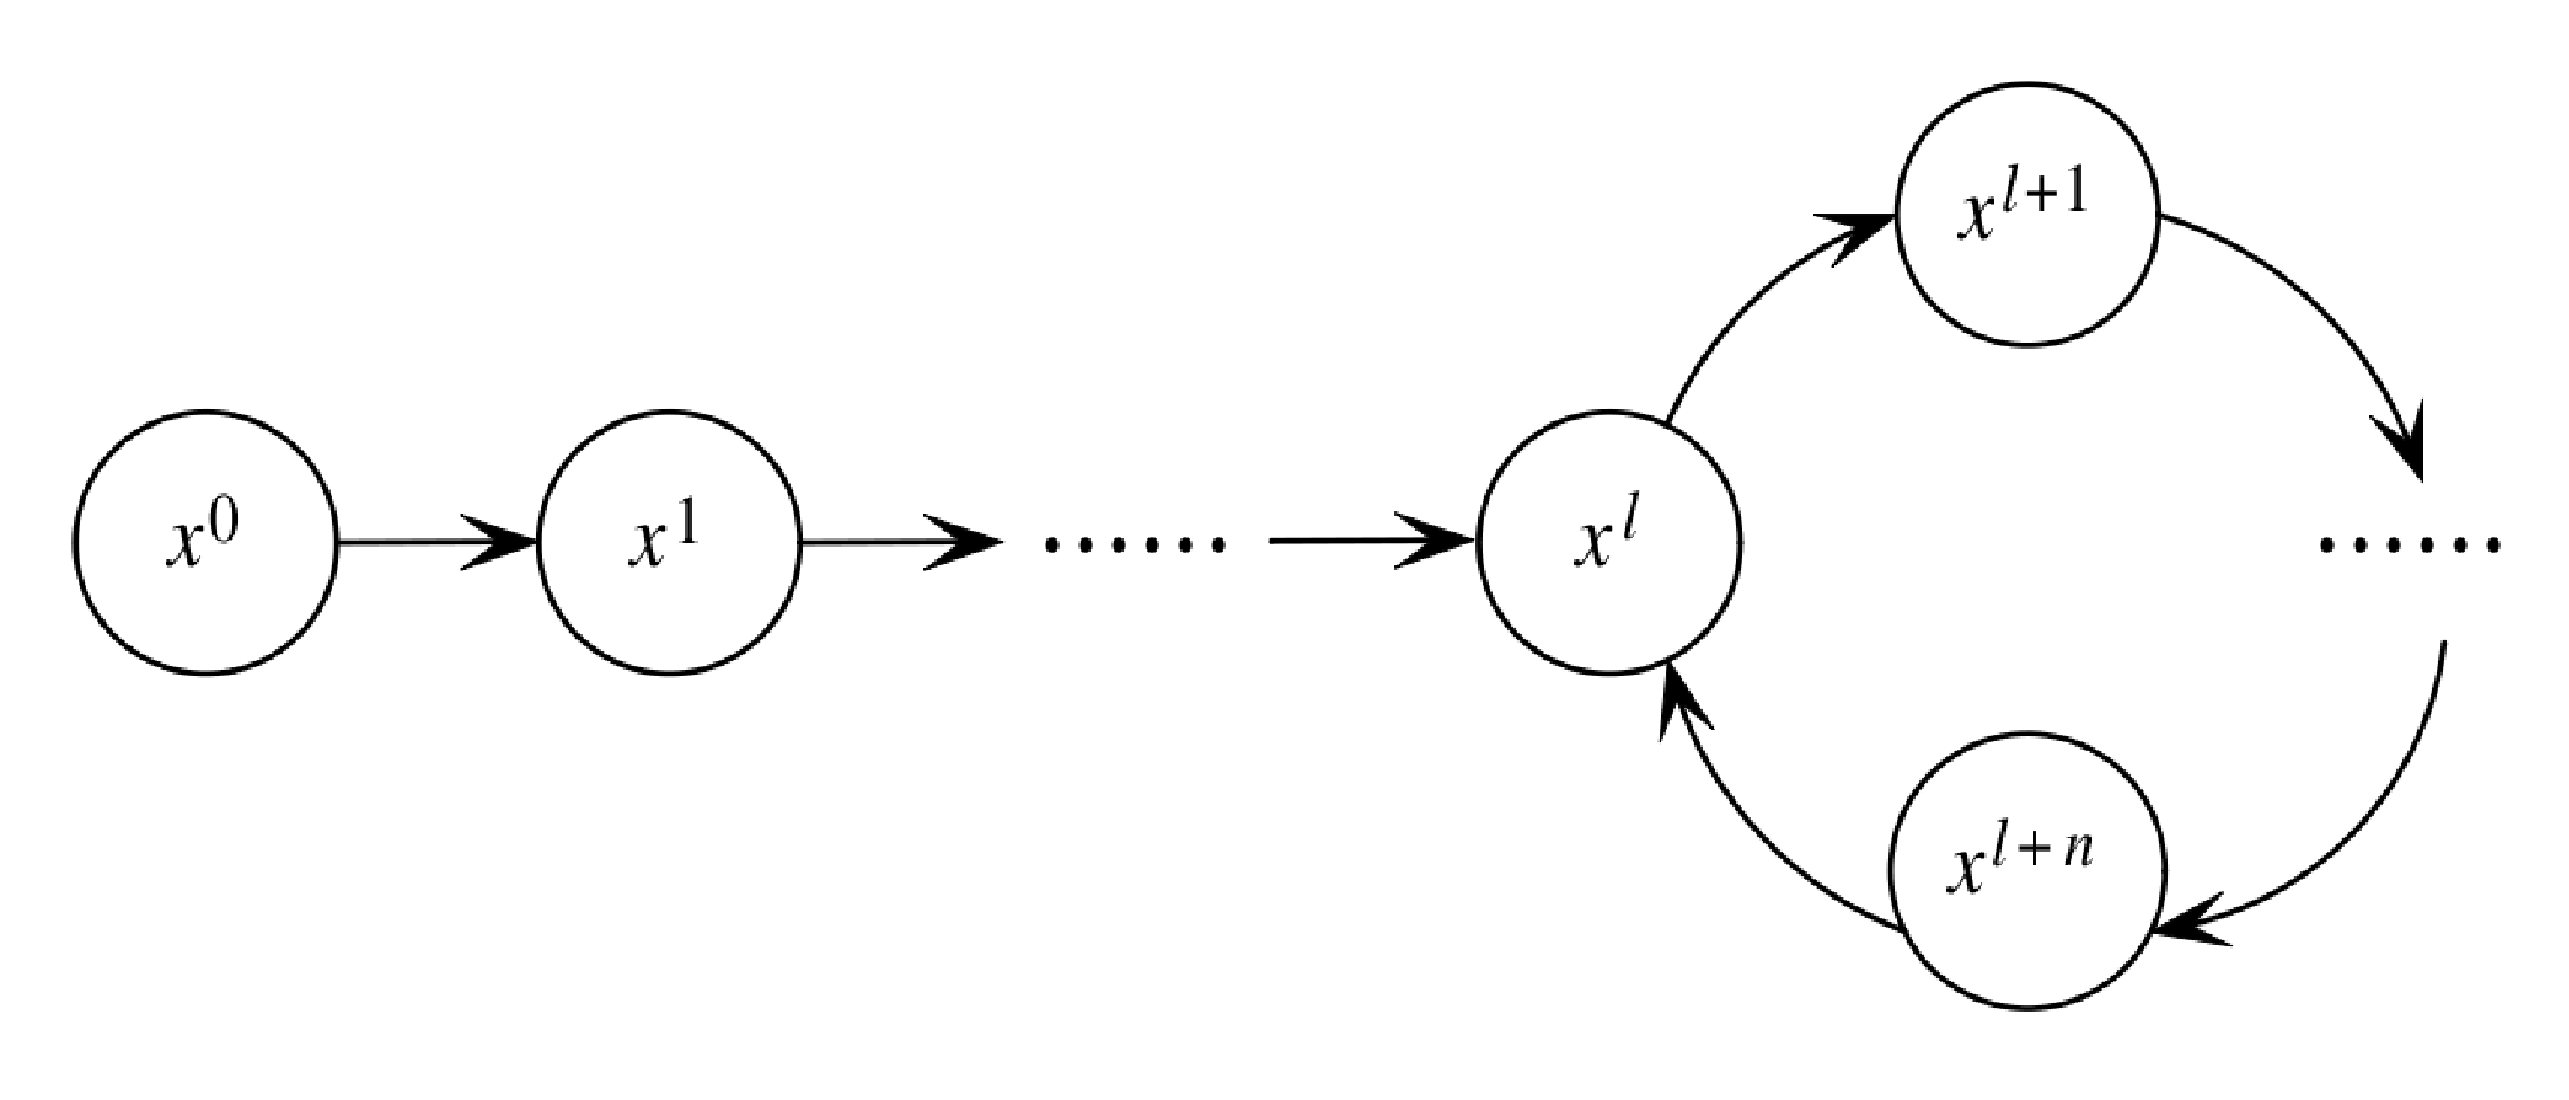
\includegraphics[scale=0.20]{pseudo_orbit.eps}
\caption{A pseudo orbit of a digital chaotic system}
\label{A pseudo orbit of a digital chaotic system}
\end{figure}

If the orbit length of $m$ and $w$ are respectively $l_m+n_m$ and $l_w+n_w$, then in an ideal situation, the transient length of the novel sequence in 4-bit output is $l_m$ (if we suppose that
$l_m \geqslant l_w$).
Table~\ref{The ideal orbit length} shows the ideal orbit length of a logistic map 
based generator and of our CIPRNG version 1 with 32-bit integers. The result 
depicts that long $l_m$ with short $n_m$ and $n_w$ make a worse orbit length.

\begin{table}
\renewcommand{\arraystretch}{1.3}
\caption{Ideal orbit length}
\label{The ideal orbit length}
\centering
% \begin{tiny}
\begin{tabular}{|c|c|c|}\toprule\hline
\multicolumn{2}{|c|}{\textbf{PRNG}}&\textbf{Ideal orbit length}\\\hline
\multicolumn{2}{|c|}{\textbf{Logistic map 1}}& $l_m+n_m$\\\hline
\multicolumn{2}{|c|}{\textbf{Logistic map 2}}& $l_w+n_w$\\\hline
\textbf{CIPRNG version 1}&\textbf{Logistic map 1+Logistic map 2}&$l_m/8+LCM(2n_mn_w,8)/8$\\\hline
\bottomrule
\end{tabular}
% \end{tiny}
\end{table}

\subsection{Security Analysis}
\label{Security Analysis Version 1 CI}
In this section the concatenation of two strings $u$ and $v$ is classically denoted by $uv$. In a cryptographic context, a pseudorandom generator is a deterministic algorithm $G$ transforming strings into strings and such that, for any seed $s$ of length m, $G(s)$ (the output of $G$ on the input $s$) has size $l_G(m)$ with $l_G(m) > m$. The notion of secure PRNGs can now be defined as follows. 

\subsubsection{Algorithm expression conversion}
For the convenience of security analysis,  Algo.\ref{Chaotic iteration} of CIPRNG version 1 is converted as in Eq.(\ref{Version 1 CI Eq}). Internal state is $x$, $S$ and $T$ are those computed by PRNG1 and PRNG2, and at each round, $x^{n-1}$ is updated to be $x^n$. 

\begin{equation}
\left\{
\begin{array}{l}
x^0 \in \llbracket 0, 2^\mathsf{N}-1 \rrbracket, S \in \llbracket 0, 2^\mathsf{N}-1 \rrbracket^\mathds{N}, T \in \llbracket 0, 2^\mathsf{N}-1 \rrbracket^\mathds{N}\\
C = S^n \& 1 + 3*\mathsf{N}\\
w^0 = {T}^m~mod~\mathsf{N}, w^1 = {T}^{m+1} \& 3, ... w^{C-1} = {T}^{m+C-1} \& 3\\ 
d^n = (1 \ll w^0) \oplus (1\ll w^1) \oplus ... (1 \ll w^{C-1})\\
\forall n \in \mathds{N}^*, x^n = x^{n-1} \oplus d^n,
\end{array}
\right.
\label{Version 1 CI Eq}
\end{equation}


\subsubsection{Proof of cryptographical security}
\label{proof1}
Let us firstly recall the following fundamental
definition.
\begin{definition}
\label{CSPRNG}
A given PRNG $G$ is cryptographically secure if for any probabilistic polynomial time algorithm $D$, for any positive polynomial $p$, and for all sufficiently large $m$'s,  
\begin{equation}
|Pr[D(G(U_m))=1]-Pr[D(U_{l_G(m)})=1]<\frac{1}{p(m)},
\end{equation}
where $U_r$ is the uniform distribution over $\{0, 1\}^r$ and the probabilities are taken over $U_m$, $U_{l_G(m)}$ as well as over the internal coin tosses of $D$.
\end{definition}

Intuitively, it means that there is no polynomial time algorithm that can distinguish a perfect uniform random generator from $G$ with a non negligible probability. Note that it is quite easily possible to change the function $l$ into any polynomial function $l'$ satisfying $l'(m)>m$.

The generation schema developed in Eq.\ref{Version 1 CI Eq} is based on $2$ pseudorandom generators. Let $H$ be the ``PRNG1'' and $I$ be the ``PRNG2''. We may assume, without loss of generality, that if for any string $S_0$ of size $L$, the size of $H(S_0)$ is $kL$,  then for any string $T_0$ of size $M$, $I(T_0)$ has a length of $kN$, where $k > 2$. It means that $l_H(N) = kL$ and $l_I(N) = kM$. Let $S_1,...,S_k$ be the string of length $L$ such that $H(S_0) = S_1 ... S_k$ and $T_1,...,T_k$ be the string of length $M$ such that $H(S_0) = T_1 ... T_k$ ($H(S_0)$ and $I(T_0)$ are the concatenations of $S_i$'s and $T_i$'s). The PRNG $X$ defined in Algo.\ref{Version 1 CI Eq} is the algorithm that maps any string $x_0S_0T_0$ of length $L+M+N$ into the string $x_0 \oplus d^1, x_0 \oplus d^1 \oplus d^2,...,(x_0 \bigoplus^{i=k}_{i=0}d^i)$ (see Eq.(\ref{Version 1 CI Eq})). One in particular has $l_X(L+M+N) = kN = l_H(N)$ and $k > M+L+N$. We announce that if $H$ is secure, then the new one from Eq.(\ref{Version 1 CI Eq}) is secure too.

\begin{proposition}
\label{cryptopreuve}
If the PRNG $H$ is a  cryptographically secure one, then $X$ is a secure cryptographic
PRNG too.
\end{proposition}

\begin{proof}
The proposition is proven by contraposition. Assume that $X$ is not
secure. By definition, there exists a polynomial time probabilistic
algorithm $D$, a positive polynomial $p$, such that for all $k_0$ there exists
$L+M+N\geq {k_0}$ satisfying 
$$| \mathrm{Pr}[D(X(U_{L+M+N}))=1]-\mathrm{Pr}[D(U_{kN}=1]|\geq \frac{1}{p(L+M+N)}.$$

Consider a word $w$ of size $kL$.
\begin{enumerate}
 \item Decompose $w$ into $w = w_1...w_k$.
 \item Pick a string $y$ of size $N$ uniformly at random.
 \item Pick a string $u$ of size $(3kN + \sum_{j=1}^{j=k}(w_j\&1)) M$.
 \item Decompose $u$ into $u = u_1...u_{3kN + \sum_{j=1}^{j=k}(w_j\&1)}$.
 \item Define $t_i = \bigoplus_{l=3N(i-1)+(\sum_{l=1}^{l=i-1}(w_j\&1))+1}^
 {j=3N(i)+(\sum_{j=1}^{j=i}(w_j\&1))}(1<<u_l)$.
 \item Compute $z = (y\oplus t_1) (y\oplus t_1 \oplus t_2) ... (y\bigoplus_{i=1}^{i=k}(t_i))$.
 \item Return $D(z)$.
\end{enumerate}


On the one hand, consider for each $y\in \mathbb{B}^{kN}$ the function $\varphi_{y}$ from $\mathbb{B}^{kN}$ into $\mathbb{B}^{kN}$ mapping $t=t_1\ldots t_k$ (each $t_i$ has length $N$) to $(y\oplus t_1 )(y\oplus t_1\oplus t_2)\ldots (y \bigoplus_{i=1}^{i=k} t_i)$.  On the other hand, treat each $u_l \in \mathbb{B}^{(3Nk + \sum_{j=0}^{j=k}(w_j\&1)) M}$ the function $\phi_{u}$ from $\mathbb{B}^{(3kN + \sum_{j=0}^{j=k}(w_i\&1)) M}$ into $\mathbb{B}^{kN}$ mapping $w = w_1 \ldots w_k$ (each $w_i$ has length $L$) to $\bigoplus_{l=1}^{l=3N+(w_1\&1)}(1<<u_l)  \bigoplus_{l=1+3N+(w_1\&1)}^{l=6N+(w_1\&1)+(w_1\&1)}(1<<u_l) \ldots \bigoplus_{l=3N(k-1)+\sum_{j=1}^{j=k-1}(w_j\&1)}^{l=3Nk+\sum_{j=1}^{j=k}(w_j\&1)}(1<<u_l)$. By construction, one has for every $w$,
\begin{equation}\label{PCH-1}
D^\prime(w)=D(\varphi_y(\phi_u(w))),
\end{equation}

Therefore, and using Eq.(\ref{PCH-1}),
one has
$\mathrm{Pr}[D^\prime(U_{kL})=1]=\mathrm{Pr}[D(\varphi_y(\phi_u(U_{kL})))=1]$, and so
\begin{equation}\label{PCH-2}
\mathrm{Pr}[D^\prime(U_{kL})=1]=\mathrm{Pr}[D(U_{kN})=1].
\end{equation}

Now, using Eq.(\ref{PCH-1}) again, one has  for every $x$,
\begin{equation}\label{PCH-3}
\mathrm{Pr}[D^\prime(U_{H(x)})=1]=\mathrm{Pr}[D(\varphi_y(\phi_u(U_{H(x)})))=1] 
\end{equation}
since where $y$ and $u_j$ are randomly generated. By construction, $\varphi_y(\phi_u(x))=X(yu_1w)$, hence 

\begin{equation}\label{PCH-4}
\mathrm{Pr}[D^\prime(H(U_{kL}))=1]=\mathrm{Pr}[D(X(U_{N+M+L}))=1]
\end{equation}

Compute the difference of Eq.(\ref{PCH-4}) and Eq.(\ref{PCH-3}), one can deduce that there exists a polynomial time probabilistic algorithm $D^\prime$, a positive polynomial $p$, such that for all $k_0$ there exists $L+M+N\geq {k_0}$ satisfying $$| \mathrm{Pr}[D^\prime(H(U_{KL}))=1]-\mathrm{Pr}[D(U_{kL})=1]|\geq \frac{1}{p(L+M+N)},$$ proving that $H$ is not secure, which is a contradiction to the first statement of this proof. 
\end{proof}

\subsection{An Efficient and Cryptographically Secure Generator Based on CIPRNG Version 1}
In Tab.\ref{Version 1 CI cs}, an efficient and cryptographically secure 
PRNG algorithm with good random qualities~\cite{bibtexwangqianxue} is given. It is based on CIPRNG version 1.

\begin{table}
\centering
\begin{tabular}{|l|l|}
\hline
~\textbf{Input}: $x$ (a 12-bit word)\\
\hline
~\textbf{Output}: $r$ (a 12-bit word)\\
\hline
~$x1 \leftarrow xorshift1();$\\
~$x2 \leftarrow xorshift2();$\\
~$x3 \leftarrow xorshift3();$\\
~$t \leftarrow bbs();$\\
~$t1 \leftarrow t \& 1;$\\
~$t2 \leftarrow t \& 2;$\\
~$t3 \leftarrow t \& 4;$\\
~$w1 \leftarrow 0;$\\
~$w2 \leftarrow 0;$\\
~$w3 \leftarrow 0;$\\
~$\textbf{While}~ i = 0 ... 11$ \\
~$w1 \leftarrow (w1 \oplus (1 \ll ((x1 \gg (i\times 2))\&3)));$\\
~$w2 \leftarrow (w2 \oplus (1 \ll ((x2 \gg (i\times 2))\&3)));$\\
~$w3 \leftarrow (w3 \oplus (1 \ll ((x3 \gg (i\times 2))\&3)));$\\
~$\textbf{EndWhile}$\\
~$\textbf{if}~(t1 \neq 0)~\textbf{then}~w1 \leftarrow (w1 \oplus (1 \ll ((x1 \gg 24)\&3)));$ \\
~$\textbf{if}~(t2 \neq 0)~\textbf{then}~w2 \leftarrow (w2 \oplus (1 \ll ((x2 \gg 24)\&3)));$ \\
~$\textbf{if}~(t3 \neq 0)~\textbf{then}~w3 \leftarrow (w3 \oplus (1 \ll ((x3 \gg 24s)\&3)));$ \\
~$x \leftarrow x \oplus w1 \oplus (w2 \ll 4) \oplus (w3 \ll 8);$\\
~$r \leftarrow x;$\\
~$\textbf{return} ~r;$\\
\hline
~\textbf{An arbitrary round of the algorithm}~\\
\hline
\end{tabular}
\caption{An efficient and cryptographically secure PRNG based on CIPRNG version}
\label{Version 1 CI cs}
\end{table}

The internal state $x$ has a size of $12$ bits. Three $32$-bit XORshift PRNGs ($xorshift1(), xorshift2(), xorshift3()$) are applied, each of them is split to $16$ $2$-bit binary blocks (value is thus between $0$ and $3$). 
 Then the $3$ LSBs (least significant bits) of the output from BBS $bbs()$ are used to decide if the $13rd$ blocks of $x1,x2, ~and ~x3$ participant the updating or not. 

According to Section~\ref{Security Analysis Version 1 CI}, this generator based on CIPRNG version 1 can turn to be cryptographically secure, if its inputted generator $I$ is cryptographically secure too. Here, $I$ is a simple BBS generator, which is one of the most secure PRNG currently available~\cite{vmd}. The $t$ value computed by $bbs()$ is obtained from
the $32$-bit long $m$, and the $log(log(m))$ LSBs of $t$ can be treated as secure. Hence, 
we can choose securely one of its $3$ LSBs.

\section{CIPRNG Version 2: a Security Proof}
\label{Security Analysis Version 2 CI}
%In this section the concatenation of two strings $u$ and $v$ is classically denoted by $uv$.
%In a cryptographic context, a pseudorandom generator is a deterministic algorithm $G$ transforming 
%strings into strings and such that, for any seed 
%$s$ of length m, $G(s)$ (the output of $G$ on the input $s$) has size $l_G(m)$ with $l_G(m) > m$. The notion of secure 
%PRNGs can now be defined as follows.

We will now make a similar proof of security for the CIPRNG version 2.

\subsection{Algorithm conversion}
For the convenience of security analysis, the CIPRNG version 2 Algorithm given in \ref{Chaotic iteration1} is also rewritten, as described in
Eq.(\ref{Version 2 CI Eq}). Internal state is $x$, $S$ and $T$ are those computed by PRNG1 and PRNG2, 
and at each round, $x^{n-1}$ is updated to $x^n$. 

\begin{equation}
\label{g}
m^n = g(S^n)=
\left\{
\begin{array}{l}
0 \text{ if }0 \leqslant{S^n}<{C^0_{32}},\\
1 \text{ if }{C^0_{32}} \leqslant{S^n}<\sum_{i=0}^1{C^i_{32}},\\
2 \text{ if }\sum_{i=0}^1{C^i_{32}} \leqslant{S^n}<\sum_{i=0}^2{C^i_{32}},\\
\vdots~~~~~ ~~\vdots~~~ ~~~~\\
N \text{ if }\sum_{i=0}^{N-1}{C^i_{32}}\leqslant{S^n}<1.\\
\end{array}
\right.
\end{equation}

We firstly recall in Eq.\ref{g} the definition of the $g$ function. Then,


\begin{equation}
\left\{
\begin{array}{l}
x^0 \in \llbracket 0, 2^\mathsf{N}-1 \rrbracket, S \in \llbracket 0, 2^\mathsf{N}-1 \rrbracket^\mathds{N}, T \in \llbracket 0, 2^\mathsf{N}-1 \rrbracket^\mathds{N}\\
m = g(S^n);\\
d^n = 0;\\
d^n = h(d^n,m,T);\\
\forall n \in \mathds{N}^*, x^n = x^{n-1} \oplus d^n,
\end{array}
\right.
\label{Version 2 CI Eq}
\end{equation}

\noindent where $h$ is defined by the Algorithm~\ref{h}.






\begin{algorithm}
\textbf{Input:} the internal state $d$, $m$, and PRNG sequence $T$\\
\textbf{output:} a state $r$\\
\begin{algorithmic}[1]
\WHILE{$i=0,\dots,m$}
\STATE$w^i\leftarrow{T^{l+i}}~mod~N$\;
    \IF{$d^n_{w^i}=0$}
    {
\STATE      $d^n_{w^i}\leftarrow{1}$\;

    }
    \ELSIF{$d^n_{w^i}=1$}
    {
\STATE      $k\leftarrow{ k+1}$\;
    }\ENDIF
\ENDWHILE
\STATE $r \leftarrow  d^n $\;
\medskip
\caption{Algorithm for $h(d,m,T)$}
\label{h}
\end{algorithmic}
\end{algorithm}


\subsection{Proof}
% \begin{definition}
% \label{CSPRNG}
% A cryptographic PRNG $G$ is secure if for any probabilistic polynomial time algorithm D, for any positive polynomial p, 
% and for all sufficiently large m's,  
% \begin{equation}
% |Pr[D(G(U_m))=1]-Pr[D(U_{l_G(m)})=1]<\frac{1}{p(m)},
% \end{equation}
% where $U_r$ is the uniform distribution over ${0, 1}^r$ and the probabilities are taken over $U_m$, 
% $U_{l_G(m)}$ as well as over the internal coin tosses of $D$.
% \end{definition}
% 
% Intuitively, it means that there is no polynomial time algorithm that can distinguish a perfect uniform 
% random generator from $G$ with a non negligible probability. Note that it is quite easily possible to change 
% the function $l$ into any polynomial function $l'$ satisfying $l'(m)>m$.

We will produce here a similar proof of security than in the previous section, 
but on the Eq.~\ref{CSPRNG} describing our CIPRNG version 2.


The generation schema developed in Algo.\ref{Chaotic iteration1} is based on $2$ pseudorandom generators. Let $H$ 
be the ``PRNG1'' and $I$ be the ``PRNG2''. 
We may assume, another time without loss of generality, that for any string $S_0$ of size $L$, if 
the size of $H(S_0)$ is $kL$, with $k > 2$, then any string $T_0$ of size $M$
has an $I(T_0)$ of size $kM$. 
It means that $l_H(L) = kL$ and $l_I(M) = kM$. 


Let $S_1,...,S_k$ be the string of length $L$ such that 
$H(S_0) = S_1 ... S_k$ and $T_1,...,T_k$ be the string of length
$M$ such that $H(S_0) = T_1 ... T_k$ ($H(S_0)$ and $I(T_0)$ are the concatenations of $S_i$'s and $T_i$'s).
The generator $X$ of Algorithm \ref{Version 2 CI Eq} maps any string of length 
$N+M+L~ x_0S_0T_0$ into the string $x_0 \oplus d^1, 
x_0 \oplus d^1 \oplus d^2,... 
(x_0 \bigoplus^{i=k}_{i=0}d^i)$ (see Eq.~\ref{Version 2 CI Eq}).
One in particular has $l_X(L+M+N) = kN = l_H(N)$ and $k > M+L+N$.
We announce that if $H$ is secure, then the generator defined in Eq.(\ref{Version 1 CI Eq}) 
is secure too.

\begin{proposition}
\label{cryptopreuve}
If $H$ is cryptographically secure PRNG, then CIPRNG version 2 is secure too.
\end{proposition}

\begin{proof}
As previously, the proposition is proven by contraposition. Assume that $X$, 
the generator defined in Eq.(\ref{Version 1 CI Eq}), is not
secure. By definition, there exists a polynomial time probabilistic
algorithm $D$ and a positive polynomial $p$, such that for all $k_0$, there exists
$L+M+N\geq {k_0}$ satisfying: 
$$| \mathrm{Pr}[D(X(U_{L+M+N}))=1]-\mathrm{Pr}[D(U_{kN}=1]|\geq \frac{1}{p(L+M+N)}.$$

\noindent Consider now a word $w$ of size $kL$.
\begin{enumerate}
 \item Decompose $w$ into $w = w_1...w_k$.
 \item Define $m=m_1m_2...m_k$ such that $m_1 = w_1~mod~N, m_2 = w_2 ~mod~N, ... m_k = w_k~mod~N$.
 \item Pick a string $y$ of size $N$ uniformly at random.
 \item Pick a string $u = {u_1,u_2...u_k}$, which is satisfied with processing $k$ times $h(0, m, u)$.
 \item Define $t_i = h(0,m_i,u_i)$.
 \item Compute $z = (y\oplus t_1) (y\oplus t_1 \oplus t_2) ... (y\bigoplus_{i=1}^{i=k}(t_i))$.
 \item Return $D(z)$.
\end{enumerate}


On one hand, consider for each $y\in \mathbb{B}^{kN}$ the function $\varphi_{y}$
from $\mathbb{B}^{kN}$ into $\mathbb{B}^{kN}$ mapping $t=t_1\ldots t_k$
(each $t_i$ has length $N$) to 
$(y\oplus t_1 )(y\oplus t_1\oplus t_2)\ldots (y
  \bigoplus_{i=1}^{i=k} t_i)$. 
 On the other hand, for each $u_l \in \mathbb{B}^{(3Nk + \sum_{j=0}^{j=k}(w_j\&1)) M}$, define the function $\phi_{u}$
 from $\mathbb{B}^{(3kN + \sum_{j=0}^{j=k}(w_i\&1)) M}$ into $\mathbb{B}^{kN}$ mapping $w = w_1 \ldots w_k$ (each 
 $w_i$ has length $L$) to 
 $\bigoplus_{l=1}^{l=3N+(w_1\&1)}(1<<u_l) \bigoplus_{l=1+3N+(w_1\&1)}^{l=6N+(w_1\&1)+(w_1\&1)}(1<<u_l) \ldots 
 \bigoplus_{l=3N(k-1)+\sum_{j=1}^{j=k-1}(w_j\&1)}^{l=3Nk+\sum_{j=1}^{j=k}(w_j\&1)}(1<<u_l)$.
 By construction, one has for every $w$,
  
\begin{equation}\label{PCH-11}
D^\prime(w)=D(\varphi_y(\phi_u(w))).
\end{equation}

Therefore, using Eq.(\ref{PCH-11}),
one has
$\mathrm{Pr}[D^\prime(U_{kL})=1]=\mathrm{Pr}[D(\varphi_y(\phi_u(U_{kL})))=1]$, and
so
\begin{equation}\label{PCH-22}
\mathrm{Pr}[D^\prime(U_{kL})=1]=\mathrm{Pr}[D(U_{kN})=1].
\end{equation}

Now, using Eq.(\ref{PCH-11}) again, one has  for every $x$,
\begin{equation}\label{PCH-33}
\mathrm{Pr}[D^\prime(U_{H(x)})=1]=\mathrm{Pr}[D(\varphi_y(\phi_u(U_{H(x)})))=1] 
\end{equation}

\noindent since $y$ and $u_j$ are randomly generated. 
By construction, $\varphi_y(\phi_u(x))=X(yu_1w)$, hence 

\begin{equation}\label{PCH-442}
\mathrm{Pr}[D^\prime(H(U_{kL}))=1]=\mathrm{Pr}[D(X(U_{N+M+L}))=1]
\end{equation}

Computing the difference of Eq.(\ref{PCH-442}) and Eq.(\ref{PCH-33}), one can deduce that
there exists a polynomial time probabilistic
algorithm $D^\prime$, a positive polynomial $p$, such that for all $k_0$ there exists
$L+M+N\geq {k_0}$ satisfying 
$$| \mathrm{Pr}[D^\prime(H(U_{KL}))=1]-\mathrm{Pr}[D(U_{kL})=1]|\geq \frac{1}{p(L+M+N)},$$
proving that $H$ is not secure, which is a contradiction. 
\end{proof}



\section{``LUT'' CIPRNG(XORshift,XORshift) Version 3}
\label{LUT CI(XORshift,XORshift) algorithms and example}
\subsection{Introduction}

The LUT (Lookup-Table) CI generator is an improved version of the CIPRNG version 2. The key-ideas are:
\begin{enumerate}
\item To use a Lookup Table for a faster generation of strategies. 
These strategies satisfy the same property than the ones provided by the decimation process.
\item And to use all the bits provided by the two inputted generators (to discard none of them).
\end{enumerate}
%Before putting these key-ideas together, we can make a first practical remark in order to improve the speed of all of our generators.
These key-ideas are put together by the following way.

%In the LUT version of the proposed generator, chaotic iterations are realized as in the Version 2 CIPRNG, in order to generate a sequence $\left(x^n\right)_{n\in\mathds{N}} \in \left(\mathds{B}^N\right)^\mathds{N}$ of Boolean vectors ($N \in \mathds{N}^*, N \geqslant 2$).
Let us firstly recall that in chaotic iterations, only the cells designed by $S^{n}-$th are ``iterated'' 
at the $n^{th}$ iteration.
$S^n$ can be either a component (\emph{i.e.}, only one cell is updated at each iteration, 
so $S^n \in \llbracket 1;N \rrbracket$) or a subset of components (any number of cells can be 
updated at each iteration, that is, $S^n \subset \llbracket 1;N \rrbracket$).
The first kind of strategies are called ``unary strategies'' whereas the second one are denoted by ``general strategies''.
In the last case, each term $S^n$ of the strategy can be represented by an integer lower than $2^N$, 
designed by $\mathcal{S}^n$, for a system having $N$ bits: the $k^{th}$ component of the system is 
updated at iteration number $n$ if and only if the $k^{th}$ digit of the binary decomposition of $\mathcal{S}^n$ is 1.
For instance, let us consider that $\mathcal{S}^n=5$, and that we iterate on a system having 6 bits ($N=6$).
As the integer 5 has a binary decomposition equal to 000101, we thus conclude that the cells number 1 and 3 
will be updated when the system changes its state from $x^{n}$ to $x^{n+1}$.
In other words, in that situation, $\mathcal{S}^n=5 \in \llbracket 0,2^6-1\rrbracket \Leftrightarrow 
S^n = \{1, 3\} \subset \llbracket 1, 6 \rrbracket$.
To sum up, to provide a general strategy of $\llbracket 1;N \rrbracket$ is equivalent to 
give an unary strategy in $\llbracket 0; 2^N-1 \rrbracket$.
Let us now take into account this remark.

Until now the proposed generators have been presented in this document by using unary 
strategies (obtained by the first inputted PRNG $S$) that are finally grouped by ``packages'' 
(the size of these packages is given by the second generator $m$): after having used each terms 
in the current package $S^{m^n},...,S^{m^{n+1}-1}$, the current state of the system is published as an output.
Obviously, when considering the CIPRNG version 2, these packages of unary strategies defined by the 
couple $(S,m)\in \llbracket 1;N \rrbracket \times \llbracket 0;N \rrbracket$ correspond to 
subsets of $\llbracket 1;N \rrbracket$ having the form $\left\{S^{m^n},...,S^{m^{n+1}-1}\right\}$, 
which are general strategies.
As stated before, these lasts can be rewritten as unary strategies that can 
be described as sequences in $\llbracket 0; 2^N-1 \rrbracket$.



The advantage of such an equivalence is to reduce the complexity of the proposed PRNG.
Indeed the LUT CIPRNG($S$,$m$) can be written as:
\begin{equation}
x^n = x^{n-1} \wedge \mathcal{S}^n.
\end{equation}
where $\mathcal{S}$ is the unary strategy (in $\llbracket 0; 2^N-1 \rrbracket$) associated 
to the couple $(S,m)\in \llbracket 1;N \rrbracket \times \llbracket 0,N \rrbracket$.

The speed improvement is obvious, the sole issue is to understand how to change $(S,m)$ by $\mathcal{S}$.
The problem to consider is that all the sequences of $\llbracket 0; 2^n-1 \rrbracket$ are not convenient.
Indeed, the properties required for the couple $(S,m)$ ($S$ must not be uniformly distributed, 
and a cell cannot be changed twice between two outputs) must be translated in requirements for 
$\mathcal{S}$ if we want to satisfy both speed and randomness.
Such constrains are solved by working on the sequence $m$ and by using some well-defined Lookup 
Tables presented in the following sections.

\subsection{Sequence $m$}
\label{LUT1}

In order to improve the speed of the proposed generator, 
the first plan is to take the best usage of the bits generated by the inputted PRNGs.
The problem is that the PRNG generating the integers of $m^n$ does not necessary takes its values 
into $\llbracket 0, N \rrbracket$, where $N$ is the size of the system.

For instance, in the CIPRNG version 2 presented previously, this sequence is obtained by a 
XORshift, which produces integers belonging into $\llbracket 0, 2^{32}-1 \rrbracket$.
However, the iterated system has 4 cells ($N=4$) in the example proposed previously thus, 
to define the sequence $m^n$, we compute the remainder modulo 4 of each integer provided by the XORshift generator.
In other words, only the last 4 bits of each 32 bits vector generated by the second XORshift are used.
Obviously this stage can be easily optimized, by splitting this 32-bits vector into 8 subsequences of 4 bits.
Thus, a call of XORshift() will now generate 8 terms of the sequence $m$, instead of only one term in the former generator.

This common-sense action can be easily generalized to any size $N \leqslant 32$ of 
the system by the procedure described in Algo.\ref{b fuction}. The idea is simply 
to make a shift of the binary vector $a$ produced by the XORshift generator, by 0, $N$, $2N$,... 
bits to the right, depending on the remainder $c$ of $n$ modulo $\lfloor N/32 \rfloor$ (that is, 
$a \gg (N \times c)$), and to take the bits between the positions $32-N$ and $32$ of this vector 
(corresponding to the right part ``$\& (2^N-1)$'' of the formula).
In that situation, all the bits provided by XORshift are used when $N$ divides 32.

\begin{algorithm}
\begin{algorithmic}[1]
\STATE $c=n~mod~\lfloor32/N\rfloor$
\IF {$c=0$}
  \STATE $a \leftarrow XORshift()$
\ENDIF

  \STATE $b^n\leftarrow (a\gg (N \times c))\& (2^N-1)$
\STATE Return {$b^n$}
\medskip
\end{algorithmic}
\caption{Generation of sequence $b^n$}
\label{b fuction}
\end{algorithm}

This Algo.\ref{b fuction} produces a sequence $(b^n)_{n \in \mathds{N}}$ of integers belonging into 
$\llbracket 0, 2^N-1 \rrbracket$.
It is now possible to define the sequence $m$ by adapting the Eq.(\ref{v2_g2}) or 
Eq.(\ref{v2_g1}) as follows.

\begin{equation}
\label{lut_m}
m^n = f(b^n)=
\left\{
\begin{array}{l}
0 \text{ if }0				\leqslant {b^n} < {C^0_N},\\
1 \text{ if }{C^0_N}	\leqslant {b^n} < \sum_{i=0}^1 {C^i_N},\\
2 \text{ if }\sum_{i=0}^1{C^i_N}	\leqslant {b^n} < \sum_{i=0}^2 {C^i_N},\\
\vdots~~~~~					~~\vdots~~~		    ~~~~\\
N \text{ if }\sum_{i=0}^{N-1} {C^i_N}	\leqslant {b^n} < 2^N.\\
\end{array}
\right.
\end{equation}

This common-sense measure can be improved another time if $N$ is not very large by using the first Lookup 
Table of this document, which is called LUT-1.
This improvement will be firstly explained through an example.

Let us consider that $N=4$, so the sequence $(b^n)_{n \in \mathds{N}}$ belongs into $\llbracket 0, 15 \rrbracket$.
The function $f$ of Eq.(\ref{lut_m}) must translate each $b^n$ into an integer $m^n \in \llbracket 0,4 \rrbracket$, 
in such a way that the non-uniformity exposed previously is respected.
Instead of defining the function $f$ analytically, a table can be given containing all the images 
of the integers into $\llbracket 0, 15 \rrbracket$ (see Tab.\ref{LUT1 for example} for instance).
As stated before, the frequencies of occurrence of the images 0,1,2, 3, and 4 must be respectively equal 
to $\frac{C_4^0}{2^4}$, $\frac{C_4^1}{2^4}$, $\frac{C_4^2}{2^4}$, $\frac{C_4^3}{2^4}$, and $\frac{C_4^4}{2^4}$.
This requirement is equivalent to demand $C_N^i$ times the number $i$, which can be translated in terms of permutations.
For instance, when $N=4$, any permutation of the list [0,1,1,1,1,2,2,2,2,2,2,3,3,3,3,4] is convenient to 
define the image of [0,1,2,...,14,15] by $f$.

This improvement is implemented in Algo.\ref{LUT1 creation}, 
which returns a table $lut1$ such that $m^n=lut1[b^n]$.

\begin{algorithm}
\caption{The LUT-1 table generation}\label{LUT1 creation}
\begin{algorithmic}[1]

    \FOR{$j=0...N$}
        \STATE $i=0$
        \WHILE{$i<C_N^j$}
             \STATE $lut1[i]=j$
             \STATE $i=i+1$
         \ENDWHILE
    \ENDFOR
\STATE Return $lut1$
\end{algorithmic}
\end{algorithm}

\begin{table*} 
\renewcommand{\arraystretch}{1.3}
\caption{A LUT-1 table for $N=4$}
\label{LUT1 for example}
\centering
  \begin{tabular}{|c|c|c|c|c|c|c|c|c|c|c|c|c|c|c|c|c|c|}
    \hline
 $b^n$  & 0 & 1 & 2 & 3 & 4 & 5 & 6 & 7 &8 &9 &10 &11 &12 &13 &14 &15\\ \hline\hline
 $m^n$ & 0 & 1 & 1 & 1 & 1 & 2 & 2 & 2 & 2 & 2 & 2 & 3 & 3 &3 & 3 &4 \\ \hline

  \end{tabular}
\end{table*}


\subsection{Defining the chaotic strategy $\mathcal{S}$ with a LUT}
\label {LUT2}
The definition of the sequence $m$ allows to determine the number of cells 
that have to change between two outputs of the LUT CI generator.
There are $C_N^m$ possibilities to change $m$ bits in a vector of size $N$.
As we have to choose between these $C_N^m$ possibilities, we thus introduce the following sequence:
\begin{equation}
w^n=XORshift2()~mod~C^m_N.
\end{equation}

With this material it is now possible to define the lookup table that provides convenient strategies to the LUT CI generator.
If the size of the system is $N$, then this table has $N+1$ columns, numbered from 0 to $N$.
The column number $m$ contains $C_N^m$ values.
All of these values have in common to present exactly $m$ times the digit 1 
and $N-m$ times the digit 0 in their binary decomposition.
The order of appearance of these values in the column $m$ has no importance, 
the sole requirement is that no column contains a same integer twice.
Let us remark that this procedure leads to several possible LUTs.

\begin{algorithm}
\caption{$LUT21$ procedure}\label{LUT2_m creation}
\begin{algorithmic}[1]
\STATE Procedure~{LUT21}{($M,N,b,v,c$)}
\STATE $count\gets c$
\STATE $value\gets v$
 \IF {$count==M$}
    \STATE $lut2[M][num] = value$
    \STATE $num = num + 1$
  \ELSE
     \FOR {$i=b....N$}
     \STATE $value = value + 2^i$
     \STATE $count = count + 1$
     \STATE  Call {recurse LUT21}{($M,N,i+1,value,count$)}
     \STATE $value = v$
     \STATE $count = c$
   \ENDFOR
 \ENDIF
\STATE End Procedure
\end{algorithmic}
\end{algorithm}

An example of such a LUT is shown in Tab.\ref{LUT2 for example}, 
when Algo.\ref{LUT2 creation} gives a concrete procedure to obtain these tables.
This procedure makes recursive calls to the function $LUT21$ defined in Algo.\ref{LUT2_m creation}.
The $LUT21$ uses the following variables.
b is used to avoid overlapping computations between two recursive calls, 
v is to save the sum value between these calls, and c counts the number of cells that have already been processed.
These parameters should be initialized as $0$.
For instance, the LUT presented in Tab.\ref{LUT2 for example} is 
the $lut2$ obtained in Algo.\ref{LUT2_m creation} with $N=4$.


\begin{algorithm}
\caption{LUT-2 generation}\label{LUT2 creation}
\begin{algorithmic}[1]

 \FOR {$i=0....N$}
    \STATE Call {LUT21}{($i,N,0,0,0$)}
  \ENDFOR
\STATE Return lut2

\end{algorithmic}
\end{algorithm}



\begin{table} 
\renewcommand{\arraystretch}{1.3}
\caption{Example of a LUT for $N=4$}
\label{LUT2 for example}
\centering
  \begin{tabular}{|l||c|c|c|c|c|}\hline
\backslashbox{$w$}{$m$}
 & $m=0$ & $m=1$ & $m=2$ & $m=3$ & $m=4$ \\ \hline\hline
$w = 0$ & 0 & 1 & 3 & 7 & 15  \\ \hline
$w = 1$ &   & 2 & 5 & 11 &   \\ \hline
$w = 2$ &   & 4 & 6 & 13 & \\ \hline
$w = 3$ &   & 8 & 9 & 14 & \\ \hline
$w = 4$ &   &   & 10 &   & \\ \hline
$w = 5$ &   &   & 12 &   &  \\ \hline
  \end{tabular}
\end{table}



\subsection{LUT CI(XORshift,XORshift) Algorithm}

The LUT CI generator is defined by the following dynamical system:
\begin{equation}
x^n = x^{n-1} \wedge \mathcal{S}^n,
\end{equation}
where $x^O\in \llbracket 0,2^N-1\rrbracket$ is a seed and $\mathcal{S}^n = lut2[w^n][m^n] = lut2[w^n][lut1[b^n]]$, 
in which $b^n$ is provided by Algo.\ref{b fuction} and $w^n=XORshift2()~mod~C^m_N$.
An iteration of this generator is written in Algo.\ref{LUT CI algo}.
 \begin{algorithm}
 \caption{LUT CI algorithm}\label{LUT CI algo}
 \begin{algorithmic}[1]


  \STATE $b^n\leftarrow PRNG1()$

    \STATE $m^n = lut1[b^n]$
    \STATE $w^n = PRNG2()$
    \STATE $S^n = lut2[m][w]$
    \STATE $x = x \wedge S^n$
    \STATE Return $x$

 \end{algorithmic}
 \end{algorithm}

\subsection{LUT CI(XORshift,XORshift) example of use}
In this example, $N = 4$ is chosen another time for easy understanding.
As before, the initial state of the system $x^0$ can be seeded by the decimal part $t$ of the current time.
With the same current time than in the examples exposed previously, we have $x^0 = ( 0, 1, 0, 0)$ (or $x^0=4$).

Algo.\ref{LUT1 creation} provides the LUT-1 depicted in Tab.\ref{LUT1 for example}.
The first XORshift generator has returned $y = 0, 11, 7, 2, 10, 4, 1, 0, 3, 9,...$.
By using this LUT, we obtain $m = 0, 3, 2, 1, 2, 1, 1, 0, 1, 2,...$.
Then the Algo.\ref{LUT2 creation} is computed, leading to the LUT-2 given by Tab.\ref{LUT2 for example}.
So chaotic iterations of Algo.\ref{LUT CI algo} can be realized, 
to obtain in this example: 0100100101010001... or 4,9,5,1...

\begin{tiny}
\begin{table} 
\centering
\begin{tabular}{|c|c|c|c|c|}
\hline
$m$ &0 & 3 &2&1  \\ \hline
$c$  & 0 & 2&5&2\\ \hline
$S$  & 0& 13&12&4  \\ \hline
$x^{0}$ & $x^{0}$ &$x^{1}$ &$x^{2}$& $x^{3}$  \\
$0$ & $0$&$1$ & $0$& $0$\\
$1$ & $1$&$0$ & $1$& $0$\\
$0$ & $0$&$0$ & $0$& $0$ \\
$0$ & $0$&$1$ & $1$& $1$\\
\hline
\end{tabular}\\
\vspace{0.5cm}
Binary Output: $x_1^{0}x_2^{0}x_3^{0}x_4^{0}x_1^{1}x_2^{1}x_3^{1}x_4^{1}x_1^{2}x_2^{2}... = 0100100101010001...$\\
Integer Output:
$x^{0},x^{1},x^{2},x^{3}... = 4,11,8,1...$
\caption{Example of a LUT CI(XORshift,XORshift) generation}
\label{lut table application example}
\end{table}
\end{tiny}

% 
\subsection{Security Analysis}
\label{Security Analysis Version 3 CI}

This CIPRNG version 3 is very similar in its design to the 
two previous versions of chaotic iterations based pseudorandom generators.
Another time, we find a mix of two inputted generators by something
that can be written as CIs.
Hence the same contraposition method could be applied 
to prove that this version 3 is cryptographically 
secure too, when its PRNG1 is secure. However, the proof
still remain to be written.


\section{The version 4 category of CIPRNGs}
\label{new version ci}
\subsection{XOR CIPRNG}
Instead of updating only one cell at each iteration as the three first versions of
our CIPRNGs, we can try to choose a subset of components and to update them together. Such an attempt leads
to a kind of merger of the two random sequences. When the updating function is the vectorial 
negation, this algorithm can be rewritten as follows~\cite{DBLP:journals/corr/abs-1112-5239}:

\begin{equation}
\left\{
\begin{array}{l}
x^0 \in \llbracket 0, 2^\mathsf{N}-1 \rrbracket, S \in \llbracket 0, 2^\mathsf{N}-1 \rrbracket^\mathds{N} \\
d^n = S^n\\
\forall n \in \mathds{N}^*, x^n = x^{n-1} \oplus d^n,
\end{array}
\right.
\label{equation Oplus1}
\end{equation}

\noindent and this rewriting can be understood as follows. The $n-$th term $S^n$ of the sequence $S$, 
which is an integer of $\mathsf{N}$ binary digits, presents
the list of cells to update in the state $x^n$ of the system (represented as an integer 
having $\mathsf{N}$ bits too). More precisely, the $k-$th
component of this state (a binary digit) changes if and only if the $k-$th digit in the 
binary decomposition of $S^n$ is 1. This generator has been called XOR CIPRNG by
the AND team, which has introduced and studied it in\cite{DBLP:journals/corr/abs-1112-5239, bfg12a:ip}.

The single basic component presented in Eq.(\ref{equation Oplus1}) is of ordinary use as a 
good elementary brick in various PRNGs. It corresponds
to the discrete dynamical system in chaotic iterations.
Such XOR CIPRNG has inspired us to introduce a more general category of CIPRNGs, presented
below.

\subsection{CIPRNG version 4: the algorithm}

It is possible to add more complexity in updating the subset 
at each iteration
in Eq.~\ref{equation Oplus1}. 
When the updating function 
is the vectorial negation, this algorithm can be written as follows (Algo.\ref{new ci}):
\begin{algorithm}
\textbf{Input:} the internal state $x$ ($\mathsf{N}$ bits)\\
\textbf{Output:} a state $r$ of $\mathsf{N}$ bits
\begin{algorithmic}[1]
\FOR{$i=1,\dots,M$}
{
\STATE$S(i)\leftarrow PRNG2\_i()$\;
}
\ENDFOR
\STATE$T \leftarrow PRNG1()$\;
\STATE$r \leftarrow x \oplus g_2(S(1),S(2),...~S(M))$,
\STATE return $r$\;
\medskip
\caption{An arbitrary round of the version 4 CI generator}
\label{new ci}
\end{algorithmic}
\end{algorithm}

$S(1), S(2), ..., S(M)$ are $M$ pseudorandom number sequences generated by $M$ XORshifts, $T^n$ is obtained by using a cryptographically secure
PRNG like the BBS. $(t_1^n,t_2^n,\dots,t_M^n)\in \{0,1\}^M$ is the binary representation of the $2^M$-bit number $T^n$.
Indeed, $(T^n)$ sequence's aim is to decimate
%A control sequence $T^n$ decimates 
the sequences %produced by the other generators 
$S(1),S(2),..., S(M)$, with a \emph{bitwise exclusive or} ($\oplus$), according to the following decimation rule:
\begin{itemize}
\item if $t^n_i = 0$, then $S^n(i)$ is discarded,
\item else $S^n(i)$ is kept for \emph{bitwise exclusive or} computing.
\end{itemize}
In brief, the produced output sequence $x^n$, based on chaotic iterations, is updated by a \emph{bitwise exclusive or} of an irregular decimation of $S(1), S(2), ..., S(M)$, according to the bits of $T^n$.


The $M$ terms $S^n(1),..., S^n(M)$ of 
the $n-$th iterate of sequences $S(1), S(2), ...,$ $S(M)$
are integers of $N$ bits. 
Each term $T^n$ of sequence $T$ is an integer having 
$M$ binary digits. 
Such a term $T^n$ presents the list of cells 
to update in the state $x^n$ of the system, which is an integer of $N$ bits too. 
This update is provided by the function $g_2(S^n(1),S^n(2), ..., S^n(M),T^n)$, 
which is defined by the Algo.\ref{g_2}. 
Indeed, each bit in $T^n$ decides whether its 
corresponding $S^n(i)$ is used in the \emph{bitwise exclusive or} computation defining $x^n$. 
More precisely, 
the $k-$th binary digit of $x^{n-1}$ changes if and only if 
the $k-$th digit in the binary decomposition of 
$g_2(S^n(1),S^n(2), ..., S^n(M),T^n)$ is 1.



\begin{algorithm}
\textbf{Input:} sequences $S^n(1), S^n(2), ..., S^n(M)$, and $T^n$\\
\textbf{output:} a state $r$ ($N$ bits)\\
\begin{algorithmic}[1]
%\STATE$b \leftarrow T^n$\;
\STATE$r \leftarrow 0 $\;
\STATE$M \leftarrow$ size of $T^n$ \;
\FOR{$i=1 \ldots M$}\;
%\STATE$c \leftarrow $\;
\IF {$T^n \& (2^{i-1}) \neq 0$}
{
\STATE $r \leftarrow r \oplus S^n(i)$\;
}\ENDIF
\ENDFOR
\STATE return $r$\;
\medskip
\caption{The $g_2(S^n(1),S^n(2),...,S^n(M),T^n)$ function}
\label{g_2}
\end{algorithmic}
\end{algorithm}


\subsection{Security Analysis}
\label{Security Analysis}
We continue to denote, in this subsection, the concatenation of two strings $u$ and $v$ by $uv$,
%In a cryptographic context, a pseudorandom generator is a deterministic algorithm $G$ transforming strings into strings and such that, for any seed 
%$s$ of length m, $G(s)$ (the output of $G$ on the input $s$) has size $l_G(m)$ with $l_G(m) > m$. The notion of secure 
%PRNGs can now be defined as follows.
% \begin{definition}
% \label{CSPRNG}
% A cryptographic PRNG $G$ is secure if for any probabilistic polynomial time algorithm D, for any positive polynomial p, 
% and for all sufficiently large m's,  
% \begin{equation}
% |Pr[D(G(U_m))=1]-Pr[D(U_{l_G(m)})=1]<\frac{1}{p(m)},
% \end{equation}
% where $U_r$ is the uniform distribution over ${0, 1}^r$ and the probabilities are taken over $U_m$, 
% $U_{l_G(m)}$ as well as over the internal coin tosses of $D$.
% \end{definition}
% 
% Intuitively, it means that there is no polynomial time algorithm that can distinguish a perfect uniform 
% random generator from $G$ with a non negligible probability. Note that it is quite easily possible to change 
% the function $l$ into any polynomial function $l'$ satisfying $l'(m)>m$. In \cite{DBLP:journals/corr/abs-1112-5239}, 
% version 3 CI has been proven that if applied PRNG is cryptographic secure, then the CIPRNG is also cryptographic secure. 
% Here, the proof for the updated version of CI (Equation~\ref{new ci}) is given.
and we consider now the Eq.(\ref{CSPRNG}) of Section~\ref{proof1}.
The generation schema developed in Algo.\ref{new ci} is based on $M+1$ pseudorandom generators. Let $H_1, 
H_2 ... H_M$ be the PRNGs that are used to update the bits of the internal state,  
and $I$ be the PRNG that decides which $H_j$ PRNG is available in this updating round. 
We may assume, without loss of generality, that for any string $S_i(j)$ of size $N$,
the size of $H_j(S_i(j))$ is $kN$. 
Then any string $T_0$ of size $M$ has $I(T_0)$ with $kM$, here $k > 2$. 
It means that $l_H(NM) = kNM$ and $l_I(M) = kM$. 

Let $S_1(1),...,S_k(2)$, $S_1(2),...,S_k(2)$, ..., $S_1(M),...,
S_k(M)$, and $T_1,...,T_k$ be the $M+1$ string sequences 
(the strings $S$ have $N$ bits whereas the string $T$  is 
constituted by $M$ bits). 
Then $H_j(S_0(j)) = S_1(j) ... S_k(j)$ and 
$I(T_0) = T_1 ... T_k$, that is, the $H_i(S(i)_0)$ are the concatenation of $S_i(j)$ and 
$T_i$. 
Using this formulation, the generator $X$ defined in Algo.\ref{new ci} is
the algorithm that maps any string $$x^0 g_2(S^1(1),S^1(2),...S^1(M),T^1)$$ of length $M+NM+N$
 into the string: 
$$
\begin{array}{l}
x^0 \oplus g_2(S^1(1),S^1(2),...,S^1(M),T^1),\\ 
x^0 \oplus g_2(S^1(1),S^1(2),...,S^1(M),T^1) \oplus g_2(S^2(1),S^2(2),...,S^2(M),T^2),\\
...,\\ 
x^0 \bigoplus^{i=k}_{i=0}g_2(S^i(1),S^i(2),...,S^i(M),T^i).
\end{array}
$$
In particular, one have $ l_X(M+NM+N) = kN = l_H(M)$, where $kN \gneq M+NM+N$.

We announce that if the PRNG $I$ is cryptographically secure, then the new one provided by Algo.\ref{new ci} 
is secure too.

\begin{proposition}
\label{cryptopreuve}
If  $I$ is a secure cryptographic PRNG, then $X$ is a secure cryptographic
PRNG too.
\end{proposition}

\begin{proof}
The proposition is proven by contraposition. Assume that $X$ is not
secure. By definition, there exists a polynomial time probabilistic
algorithm $D$ and a positive polynomial $p$, such that for all $k_0$ there exists
$M+NM+N \geq k_0$ satisfying 
$$| \mathrm{Pr}[D(X(U_{M+NM+N}))=1]-\mathrm{Pr}[D(U_{kN}=1)]|\geq \frac{1}{p(M+NM+N)}.$$
We describe a new probabilistic algorithm $D^\prime$ on inputs $W$ 
(each is of size $kM$):
\begin{enumerate}
\item Decompose $w$ into $w=w_1\ldots w_{k}$.
\item Pick a string $y$ of size $N$ uniformly at random.
\item Pick $M$ strings of size $kN$: $u(1),...,u(M)$.
\item Decompose each $u(j)$ into $u(j) = u_1(j) \ldots u_k(j)$.
\item Define $t_i= \bigoplus_{j=0}^{j=M-1}((w_i>>j)\&1)\times u_{i}(j+1))$ from Algo.\ref{g_2};
\item Compute $z=(y\oplus t_1)(y\oplus t_1 \oplus t_2)...(y \bigoplus_{i=1}^{i=k}(t_i))$.
\item Return $D(z)$.
\end{enumerate}


Consider for each $y\in \mathbb{B}^{kN}$ the function $\varphi_{y}$
from $\mathbb{B}^{kN}$ into $\mathbb{B}^{kN}$ mapping $t=t_1\ldots t_k$
(each $t_i$ has length $N$) to 
$(y\oplus t_1 )(y\oplus t_1\oplus t_2)\ldots (y
  \bigoplus_{i=1}^{i=k} t_i)$. By construction, one has for every $t$,
\begin{equation}\label{PCH-14}
D^\prime(w)=D(\varphi_y(t)),
\end{equation}
where $y$ is randomly generated. 
Moreover, for each $y$, $\varphi_{y}$ is injective: if 
$$(y\oplus t_1)(y\oplus t_1\oplus t_2 ) \ldots (y\bigoplus_{i=1}^{i=k_1}
t_i )=(y\oplus t_1^\prime)(y\oplus t_1^\prime\oplus t_2^\prime)\ldots
(y\bigoplus_{i=1}^{i=k} t_i^\prime),$$ then for every $1\leq j\leq k$,
$y\bigoplus_{i=1}^{i=j} t_i^\prime=y\bigoplus_{i=1}^{i=j} t_i$. It follows,
by a direct induction, that $t_i=t_i^\prime$.
Consider also for each $u_i(j) \in \mathbb{B}^{kN}$ 
the function $\phi_u$
from $\mathbb{B}^{kN}$ into $\mathbb{B}^{kN}$ mapping $w=w_1\ldots w_k$ 
(each $w_i$ has length $M$) to: 

\noindent $\bigoplus_{j=0}^{j=M-1}((w_1>>j)\&1)\times u_{1}(j+1)\bigoplus_{j=0}^{j=M-1}((w_2>>j)\&1)\times u_{2}(j+1)$

\noindent $...\bigoplus_{j=0}^{j=M-1}((w_k>>j)\&1)\times u_{k}(j+1)$. 

The $u_i(j)$ is generated by $H(j)$ PRNG and $\phi_u$ is injective, so if 

\noindent $\bigoplus_{j=0}^{j=M-1}((w_1>>j)\&1)\times u_{1}(j+1))\bigoplus_{j=0}^{j=M-1}((w_2>>j)\&1)\times u_{2}(j+1))$

\noindent $\ldots \bigoplus_{j=0}^{j=M-1}((w_k>>j)\&1)\times u_{k}(j+1))$ 

\noindent = $\bigoplus_{j=0}^{j=M-1}((w_1^\prime>>j)\&1)\times u_{1}(j+1))\bigoplus_{j=0}^{j=M-1}((w_2^\prime>>j)\&1)\times u_{2}(j+1))$

\noindent $\ldots \bigoplus_{j=0}^{j=M-1}((w_k^\prime>>j)\&1)\times u_{k}(j+1)),$

\noindent then $w_i = w^\prime_i$ can be found.
So, according to 
Eq.(\ref{PCH-14}):
\begin{equation}\label{PCH-114}
D^\prime(w)=D(\varphi_y(\phi_u(w))),
\end{equation}

Furthermore, using Eq.(\ref{PCH-114}),
one has
$\mathrm{Pr}[D^\prime(U_{kM})=1]=\mathrm{Pr}[D(\varphi_y(\phi_u(U_{kM})))=1]$ and,
therefore, 
\begin{equation}\label{PCH-24}
\mathrm{Pr}[D^\prime(U_{kM})=1]=\mathrm{Pr}[D(U_{kM})=1].
\end{equation}

Now, using Eq.(\ref{PCH-114}) again, one has  for every $x$,
\begin{equation}\label{PCH-34}
D^\prime(I(x))=D(\varphi_y(\phi_u(I(x)))),
\end{equation}
since $y$ and all $u(j)$ are randomly generated. 
By construction, $\varphi_y(\phi_u(I(x)))=X(yxu(1)...u(M))$, hence
\begin{equation}\label{PCH-44}
\mathrm{Pr}[D^\prime(I(U_{M}))=1]=\mathrm{Pr}[D(X(U_{M+NM+N}))=1].
\end{equation}

Using Eq.(\ref{PCH-44}) minus Eq.(\ref{PCH-24}), one can deduce that
there exists a polynomial time probabilistic
algorithm $D^\prime$, a positive polynomial $p$, such that for all $k_0$ there exists
$M+NM+N \geq k_0$ satisfying
$$| \mathrm{Pr}[D^\prime(I(U_{M}))=1]-\mathrm{Pr}[D^\prime(U_{kM}=1)]|\geq \frac{1}{p(M+NM+N)},$$
proving that $I$ is not secure, which is a contradiction. 
\end{proof}

\subsection{Efficient cryptographic secure PRNG based on CI}
\label{prng fpga}
Tab.\ref{fpga ci} describes an efficient, chaotic, and cryptographically secure 
PRNG having a perfect statistical profile.
Its can be divided into two parts, as explained below. 


The first part is based on Algo.\ref{new ci}.
This part is very suitable for FPGA as it can be easily 
arranged to be processed in parallel.
Additionally, as stated in the previous section, 
%more than that, according to the description of Section~\ref{Security Analysis}, 
this new version of our CIPRNG can turn to be cryptographically secure.
To obtain such a secured CIPRNG,
%For constructing the generator which is cryptographic secure, 
$M + 1$ generators must be provided as input, one of them being
cryptographically secure.
In the proposed design, the BBS secured generator has been chosen 
due to its simplicity. 
Due to its slowness, this BBS is used to compute the $T$ sequence of Algo.\ref{new ci}.
The size of $m$ is 32 bits. 
It is well known that the $log(log(m))$ least significant bits 
can be securely extracted at each iteration of the BBS~\cite{vmd}.
So we set $M = 3$, leading to the selection of 2 XORshifts 
playing the role of $S$. They are denoted $XORshift1$ and $XORshift2$ 
in Tab.\ref{fpga ci}. 
Each XORshift output is separated into two $32$ bits blocks, leading to 
four $32$ bits numbers. 
Three of them (namely, the two $32$ bits blocks of $XORshift1$ 
and the first one of $XORshift2$) are controlled by the bits outputted
by the BBS according to Algo.\ref{new ci}.
The last $32$ bits block, on its part, is used in the second part of the algorithm.
More precisely, if one bit in the $bbs$ output is $0$, then the corresponding 
$32$ bits number is not used during the \emph{exclusive or} processing, 
whereas it is considered if this BBS bit is $1$.
% On the contrary, 
%if the considered bit is $1$, such bits would be exclusive-or with the state.

\begin{table}
\caption{Efficient pseudorandom generator designed for FPGAs}
\centering
\begin{tabular}{|l|l|}
\hline
~\textbf{Input}: $x$ (a 32-bit word)\\
\hline
~\textbf{Output}: $r$ (a 32-bit word)\\
\hline
~$t1 \leftarrow XORshift1();$\\
~$t2 \leftarrow XORshift2();$\\
~$t4 \leftarrow bbs();$\\
~\textbf{if} $t4 \& 1 \neq 0;$ \textbf{then} $x \leftarrow x \oplus (t1 \& 0x0ffffffff);$\\
~\textbf{if} $t4 \& 2 \neq 0;$ \textbf{then} $x \leftarrow x \oplus (t1 >> 32);$\\
~\textbf{if} $t4 \& 4 \neq 0;$ \textbf{then} $x \leftarrow x \oplus (t2 \& 0x0ffffffff);$\\
~$x \leftarrow x \oplus (t2 >> 32);$\\
~$r \leftarrow x;$\\
~\textbf{return} $r;$\\
\hline
~\textbf{An arbitrary round of the algorithm}~\\
\hline
\end{tabular}
\label{fpga ci}
\end{table}

According to our experiments, the sole first part of the algorithm cannot 
produce a statistically perfect output. This is not contradictory with
Prop.~\ref{cryptopreuve}, as the cryptographically secure property
is an asymptotic one.
Following the approach detailed in~\cite{bfg12a:ip}, 
we have used the chaotic iterations to improve the 
statistical behavior of the proposed generator.
Hence, the second part of the algorithm consists 
in using the last $32$ bits block of $XORshift2$ 
to realize Eq.(\ref{equation Oplus1}) on the output 
of the first part. 
By doing so, we obtain in 
Tab.\ref{fpga ci} a generator being
both chaotic and cryptographically secure~\cite{DBLP:journals/corr/abs-1112-5239}.

This algorithm has a very similar design than to the efficient GPU CI version
presented in~\cite{DBLP:journals/corr/abs-1112-5239}, which has 
successfully passed the stringent TestU01 battery of statistical 
tests~\cite{Lecuyer2009}.
However, in the GPU version, no BBS is used to determine which bits
in the most significant binary block of size 32 of XORshift
will be used in the process. Moreover, the number of used XORshifts
is not the same in this cryptographically secured generalization 
of the generators formerly described in~\cite{DBLP:journals/corr/abs-1112-5239}. 
